
\noindent 
\textbf{\stepcounter{zadatak}
\thecjelina.\thezadatak.}
Na slici dolje prikazan je sustav od dva bloka mase $m_A=3\ kg$ i $m_B=6\ kg$ koji su povezani tankom nerastezljivom niti. Kut $\beta=60^\circ $, koeficijent kinetičkog trenja između blokova i podloge iznosi $\mu_k=0,1$, a trenje na koloturi se zanemaruje. Koliki je iznos sile napetosti niti?
\begin{figure}[ht]%{r}{0.7\textwidth} % Inline image example
  \begin{center}
    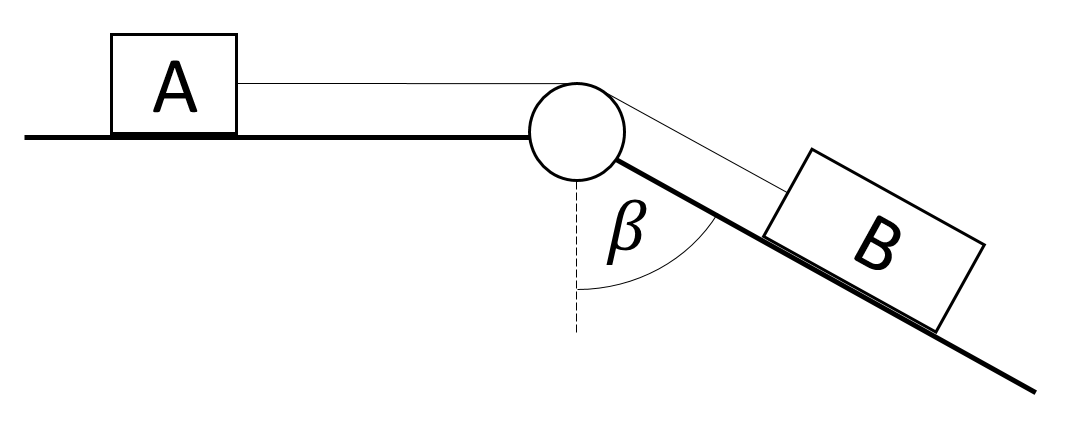
\includegraphics[scale=0.20]{03_Dinamika_materijalne_tocke/zadatak_D735.png}
  \end{center}
  %\caption{Fish}
\end{figure}

